%%%%%%%%%%%%%%%%%%%%%%%%%%%%%%%%%%%%%%%%%%%%%%%%%%%%%%%%%%%%%%%%%%%%
\section{Organization and Management}
\label{sec:fdgen-slow-cryo-org}
% sowjanya

%%%%%%%%%%%%%%%%%%%%%%%%%%%%%%%%%%%
\subsection{Slow Controls and Cryogenics Instrumentation Consortium Organization}
\label{sec:fdgen-slow-cryo-org-consortium}

% same in sp and dp

The organization of the \dword{cisc} consortium is shown in
Figure~\ref{fig:gen-slow-cryo-org}. The \dword{cisc} consortium board is
currently formed from institutional representatives from \num{17} institutes
as shown in Table~\ref{tab:gen-slow-cryo-org}. The consortium leader
acts as the spokesperson for the consortium and is responsible for the
overall scientific program and management of the group. The technical
leader of the consortium is responsible for the project management for
the group.  Currently five working groups are envisioned in the
consortium (leaders to be appointed):


%Cryogenics systems gas analyzers, liquid level monitors and cryogenic internal piping; CFD simulations

%\lar instrumentation purity monitors, thermometers, cameras and light emitting system, and instrumentation test facility; feedthroughs; \efield simulations; Instrumentation precision studies; \dword{protodune} data analysis coordination efforts




\begin{description}
 \item[Cryogenics Systems] gas analyzers, liquid level
  monitors and cryogenic internal piping; CFD simulations
 \item[\lar Instrumentation] purity monitors, thermometers,
   cameras and lightemitting system, and instrumentation test facility;
   feedthroughs; \efield simulations;
   instrumentation precision studies;
   \dword{protodune} data analysis coordination efforts
 \item [Slow Controls Base Software and Databases]  Base software, alarms and archiving databases, and monitoring tools;
   variable naming convention and slow controls quantities
 \item [Slow Controls Detector System Interfaces] Signal processing software and hardware interfaces (e.g., power supplies);
   firmware; rack hardware and infrastructure   
 \item [Slow Controls External Interfaces] Interfaces with external detector systems (e.g., cryogenics system, beam, facilities, \dword{daq})
\end{description}

\begin{dunefigure}[\dword{cisc} consortium organization]{fig:gen-slow-cryo-org}
{\dword{cisc} consortium organizational chart}
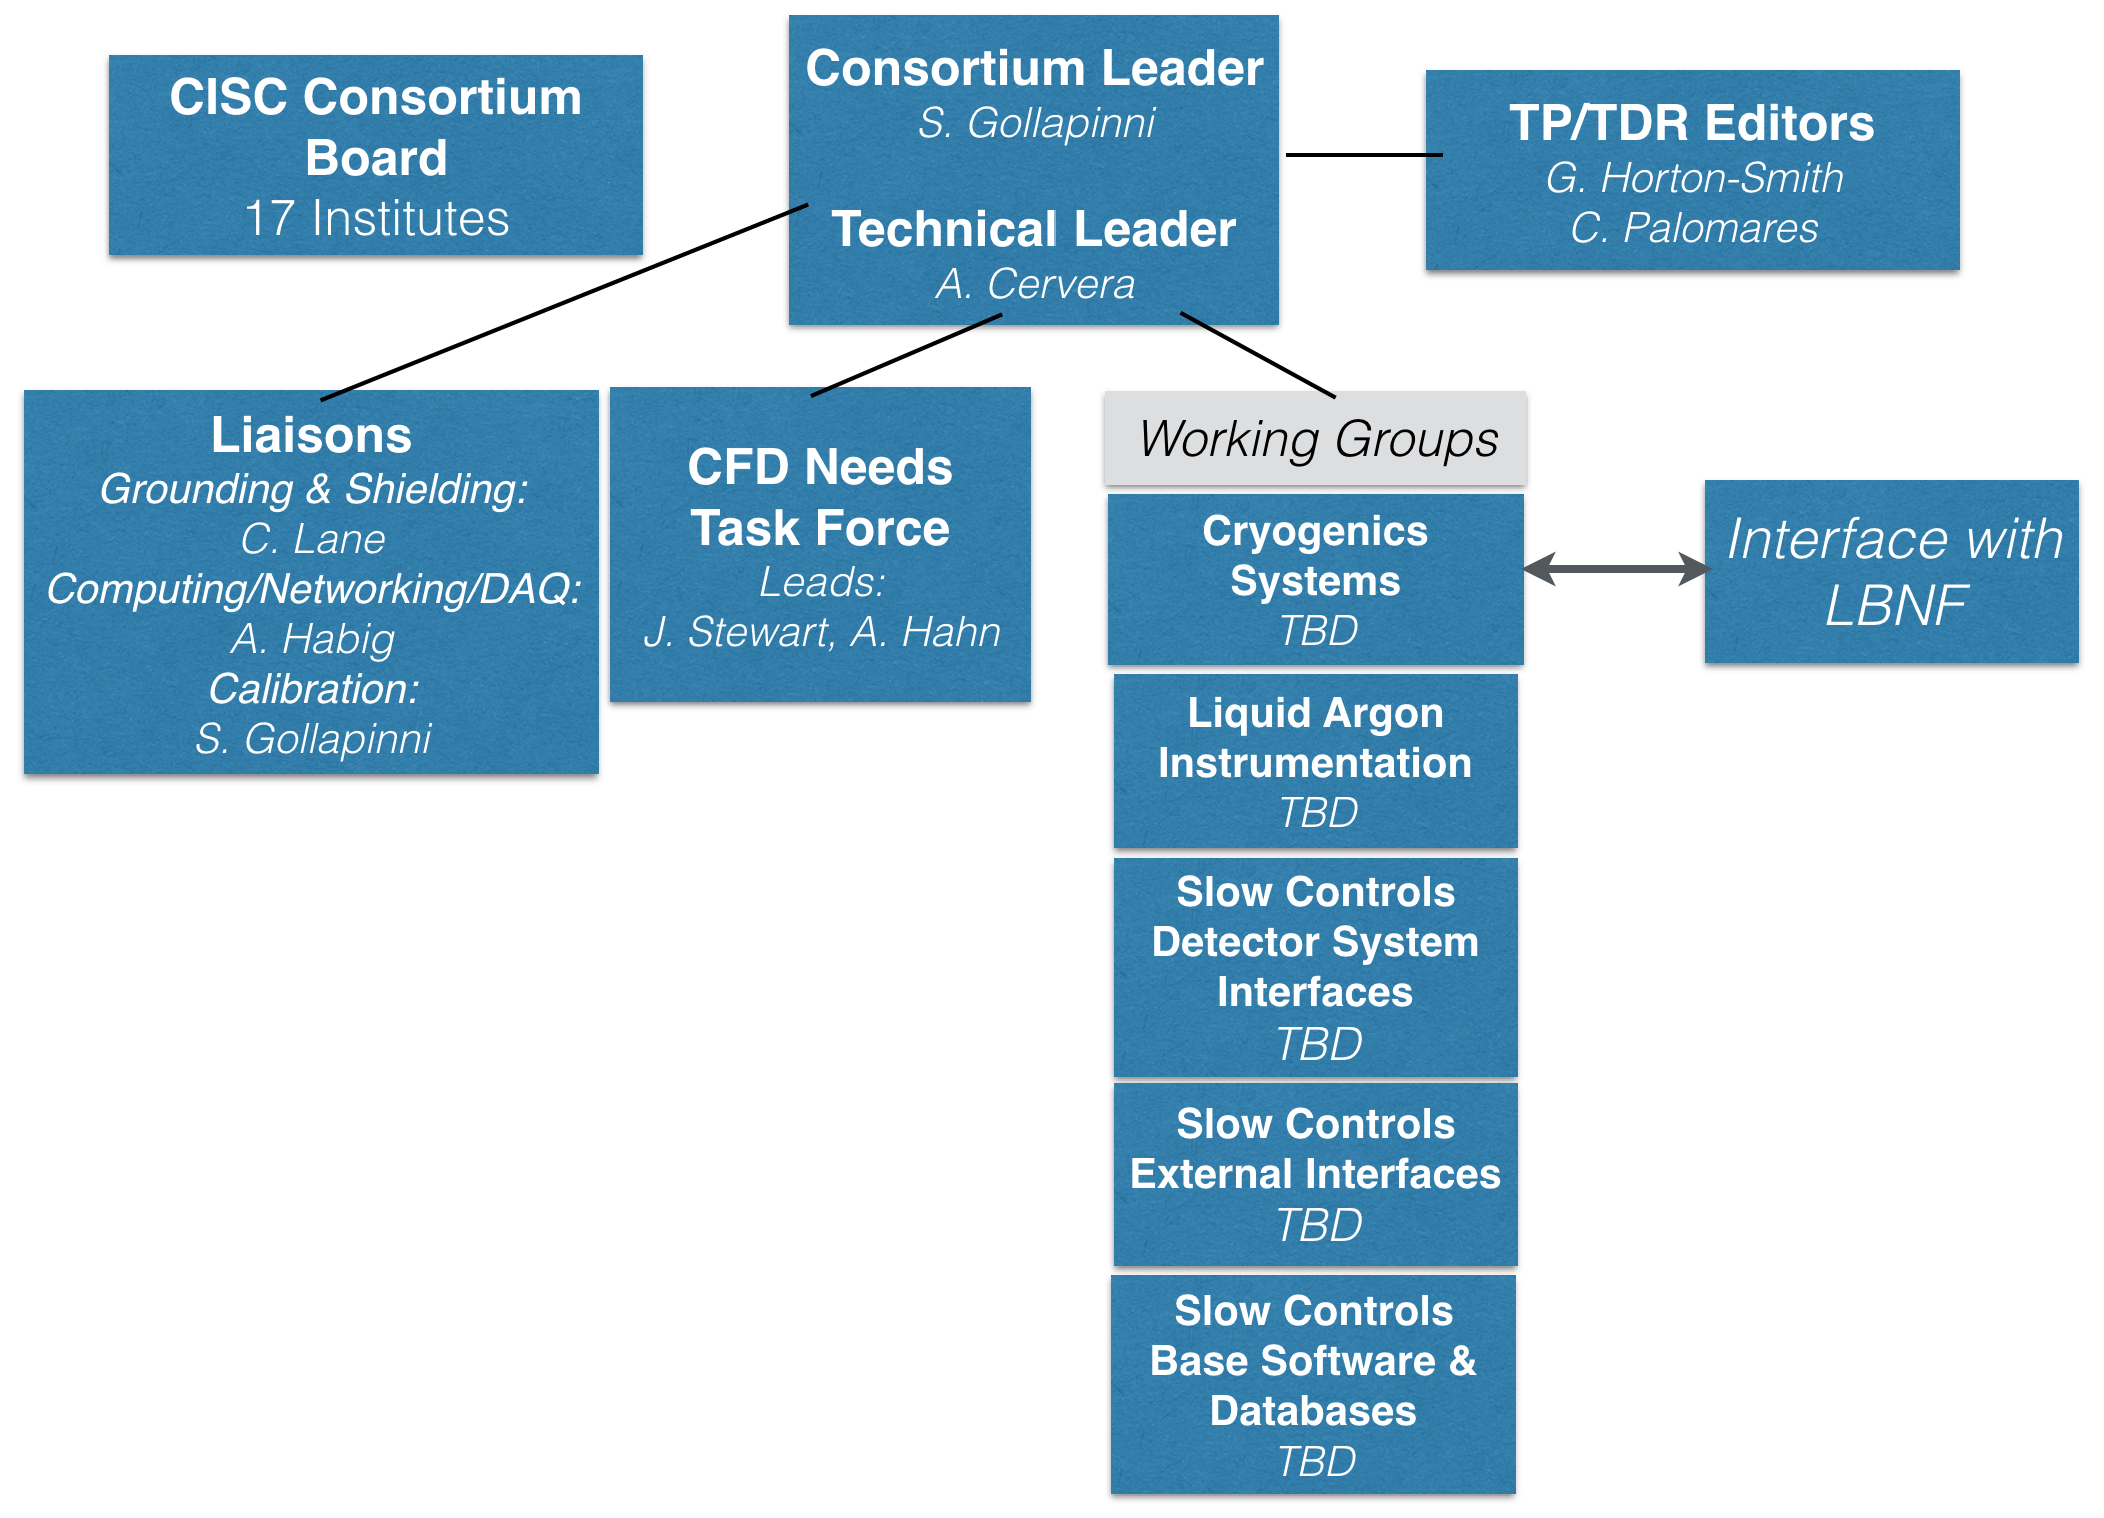
\includegraphics[width=0.7\textwidth]{cisc_org}
\end{dunefigure}

Additionally, since the \dword{cisc} consortium broadly interfaces with other
groups, liaisons have been identified for various roles as listed in
Figure~\ref{fig:gen-slow-cryo-org}. A short-term focus group was
recently formed to understand the needs for cryogenics modeling for the
consortium. The Technical Proposal (TP) and \dword{tdr}
editors are responsible for the overall editing and delivery of
these documents to the collaboration. Currently members from new
institutes are added to the consortium based on consensus from the
consortium board members.

\begin{dunetable}
[\dword{cisc} Consortium Institutions]
{p{0.3\textwidth}p{0.2\textwidth}p{0.3\textwidth}}
{tab:gen-slow-cryo-org}
{Current \dword{cisc} Consortium Board Members and their institutional affiliations}
Member Institute  &  Country  &  Consortium Board Representative \\ \toprowrule
CIEMAT  &  Spain  &  Ines Gil Botella \\ \colhline
Instituto de Fisica Corpuscular  &  Spain  &  Anselmo Cervera \\ \colhline
University of Warwick  &  United Kingdom  &  Gary Barker \\ \colhline
University College London  &  United Kingdom  &  Mario Campanelli \\ \colhline
Argonne National Lab  &  USA  &  Jim Grudzinski  \\ \colhline
Brookhaven National Lab  &  USA  &  Jim Stewart \\ \colhline
University of California (Irvine)  &  USA  &  Jianming Bian \\ \colhline
Drexel University  &  USA  &  Charles Lane \\ \colhline
Fermi National Accelerator Lab  &  USA  &  Alan Hahn \\ \colhline
University of Hawaii  &  USA  &  Jelena Maricic \\ \colhline
University of Houston  &  USA  &  Andrew Renshaw \\ \colhline
Idaho State University  &  USA  &  Ed Tatar \\ \colhline
Kansas State University  &  USA  &  Glenn Horton-Smith \\ \colhline
University of Minnesota (Duluth)  &  USA  &  Alec Habig \\ \colhline
Notre Dame University  &  USA  &  John LoSecco \\ \colhline
University of Tennessee at Knoxville  &  USA  &  Sowjanya Gollapinni \\ \colhline
Virginia Tech &		USA	&	Camillo Mariani \\
\end{dunetable}


%%%%%%%%%%%%%%%%%%%%%%%%%%%%%%%%%%
\subsection{Planning Assumptions}
\label{sec:fdgen-slow-cryo-org-assmp}

The slow controls and cryogenic instrumentation will be a joint effort for \single and \dual{}.
A single slow controls system will be implemented to serve both \single and \dual{}.

Design and installation of cryogenics systems (gas analyzers, liquid level monitoring, internal piping) will be coordinated with LBNF, with the consortium providing resources, and effort and expertise provided by LBNF.
\dword{protodune} designs for \lar instrumentation (purity monitors, thermometers, cameras, test facility) will be the basis for DUNE designs. Design validation, testing, calibration, and performance will be evaluated through \dword{protodune} data.

% %%%%%%%%%%%%%%%%%%%%%%%%%%%%%%%%%%%
% The editors at meeting of 2/13 suggest that the WBS section should be deleted in the TP. Accordingly, I have commented it out.
% \subsection{WBS and Responsibilities}
% \label{sec:fdgen-slow-cryo-org-wbs}


%%%%%%%%%%%%%%%%%%%%%%%%%%%%%%%%%%
% The editors at meeting of 2/13 suggest that the TP need not have costing. Accordingly, I have renamed this section ``High-level Schedule''.
\subsection{High-level Schedule}
\label{sec:fdgen-slow-cryo-org-cs}

Table \ref{tab:fdgen-slow-cryo-schedule} shows key milestones on
the path to the \dword{tdr} and CD-2. \fixme{DOE-specific} The first two milestones have been met by the consortium.
The consortium has made good progress on the third milestone and is currently working to develop support structure designs.

\begin{dunetable}
[Key \dword{cisc} Milestones leading to \dword{tdr}]
{p{0.15\linewidth}p{0.60\linewidth}}
{tab:fdgen-slow-cryo-schedule}
{Key \dword{cisc} Milestones leading to \dword{tdr}.}   
Date & Milestone \\ \toprowrule
Dec.\ 2017 & Finalize \single cryostat instrumentation \fdth{}s \\ \colhline
Dec.\ 2017 & Develop a baseline conceptual design/layout for the internal cryogenic piping \\ \colhline
Mar.\ 2018 & Develop conceptual designs (including support structure) for all instrumentation devices \\ \colhline
Apr.\ 2018 & PrM design performance metrics for the \dword{spmod} from \dword{pdsp} PrM tests in \lar \\ \colhline
May   2018 & Define slow controls hardware/software requirements and layout \\ \colhline
May   2018 & Technical Proposal \\ \colhline
Aug.\ 2018 & Use \dword{pdsp} instrumentation/operations data to validate designs \\ \colhline
Nov.\ 2018 & Finish producing needed \efield and CFD simulations \\ \colhline
Dec.\ 2018 & Full design of the cryogenics instrumentation test facility \\ \colhline
Jan.\ 2019 & Develop a complete architectural design for slow controls \\ \colhline
Feb.\ 2019 & Finalize designs all instrumentation devices \\ \colhline
Apr.\ 2019 & \dword{tdr} \\ \colhline
Oct.\ 2019 & CD-2 DOE Review \\
\end{dunetable}

